\documentclass{article}

\usepackage[english]{babel}

% Set page size and margins
% Replace `letterpaper' with `a4paper' for UK/EU standard size
\usepackage[letterpaper,top=2cm,bottom=2cm,left=3cm,right=3cm,marginparwidth=1.75cm]{geometry}
\usepackage{graphicx}

\title{Research Automation White Paper}
\author{Shiro Takagi}

\begin{document}
\maketitle

\section{What is Research?}

\subsection{The Working Definition of Research}
Research is the act of generating new knowledge. In other words, it can be thought of as an endeavor to make the unknown known.

\subsection{The Patterns in Research}

It is believed that research began with individual and concrete tasks. Among them, common actions were patterned and crystallized as a scientific method. We currently recognize this abstract set of behaviors as research. For example, hypothetico-deductive method and hypothesis testing are abstracted scientific method.

Also, researchers use a research paper as a medium of knowledge transfer. Therefore, there are patterned activities related to a research paper. Examples of these include conducting surveys, gathering information from papers, and writing a thesis.

Note that these are necessary tasks just because we use a paper as a medium of knowledge transfer, but they may not necessarily be indispensable for generating new knowledge. There are other such tasks as well. For example, peer review and fund raising are essential to current research practices in society, but they may not necessarily be indispensable for knowledge production.

In this way, various tasks arise in conjunction with research. When considering the automation and optimization of research, it is desirable to consider streamlining all of these tasks. However, in this article, we focus on the process from determining a research topic to publishing a research paper. We will refer to this process simply as the \textit{research process} from here on.

\subsection{Research Process}

\subsubsection{Overview}

As mentioned earlier, research is an attempt to turn the unknown into the known. Therefore, the research process can be seen as a function that takes the unknown as input and outputs the known. However, in reality, a single research paper may not be enough to turn the unknown into the known. Therefore, in practice, the research process is considered to be a procedure that takes the unknown as input, and outputs a text that describes the procedures and their results, as well as their interpretation, in order to turn the unknown into the known.

First, let me structure the common research process. In particular, I will base the structuring of the research process on the method of empirical science, which many researches rely on as a foundation. However, I believe that this framework can be applied to other research activities, such as mathematics, as well. I will explain the reason for this later.

The research process, especially that of empirical science, is carried out through the following steps: topic decision, hypothesis generation, verification design, verification, and analysis of experimental results. The outputs of these steps are then written into a paper, which undergoes peer review and is eventually published.

Note that some commonly seen items, such as surveys, are not included here for a reason. First, as mentioned earlier, gathering information from papers is only a means of knowledge transfer through the use of a thesis. Second, information extraction from papers can be done at any stage of the research process. Thus, I believe that processing related to a paper, such as \textit{reading papers} and \textit{writing a paper}, needs to be considered separately from the aforementioned research process.

Taking all of this into account, the research process can be expressed as follows:

\begin{figure}[htb]
    \centering
    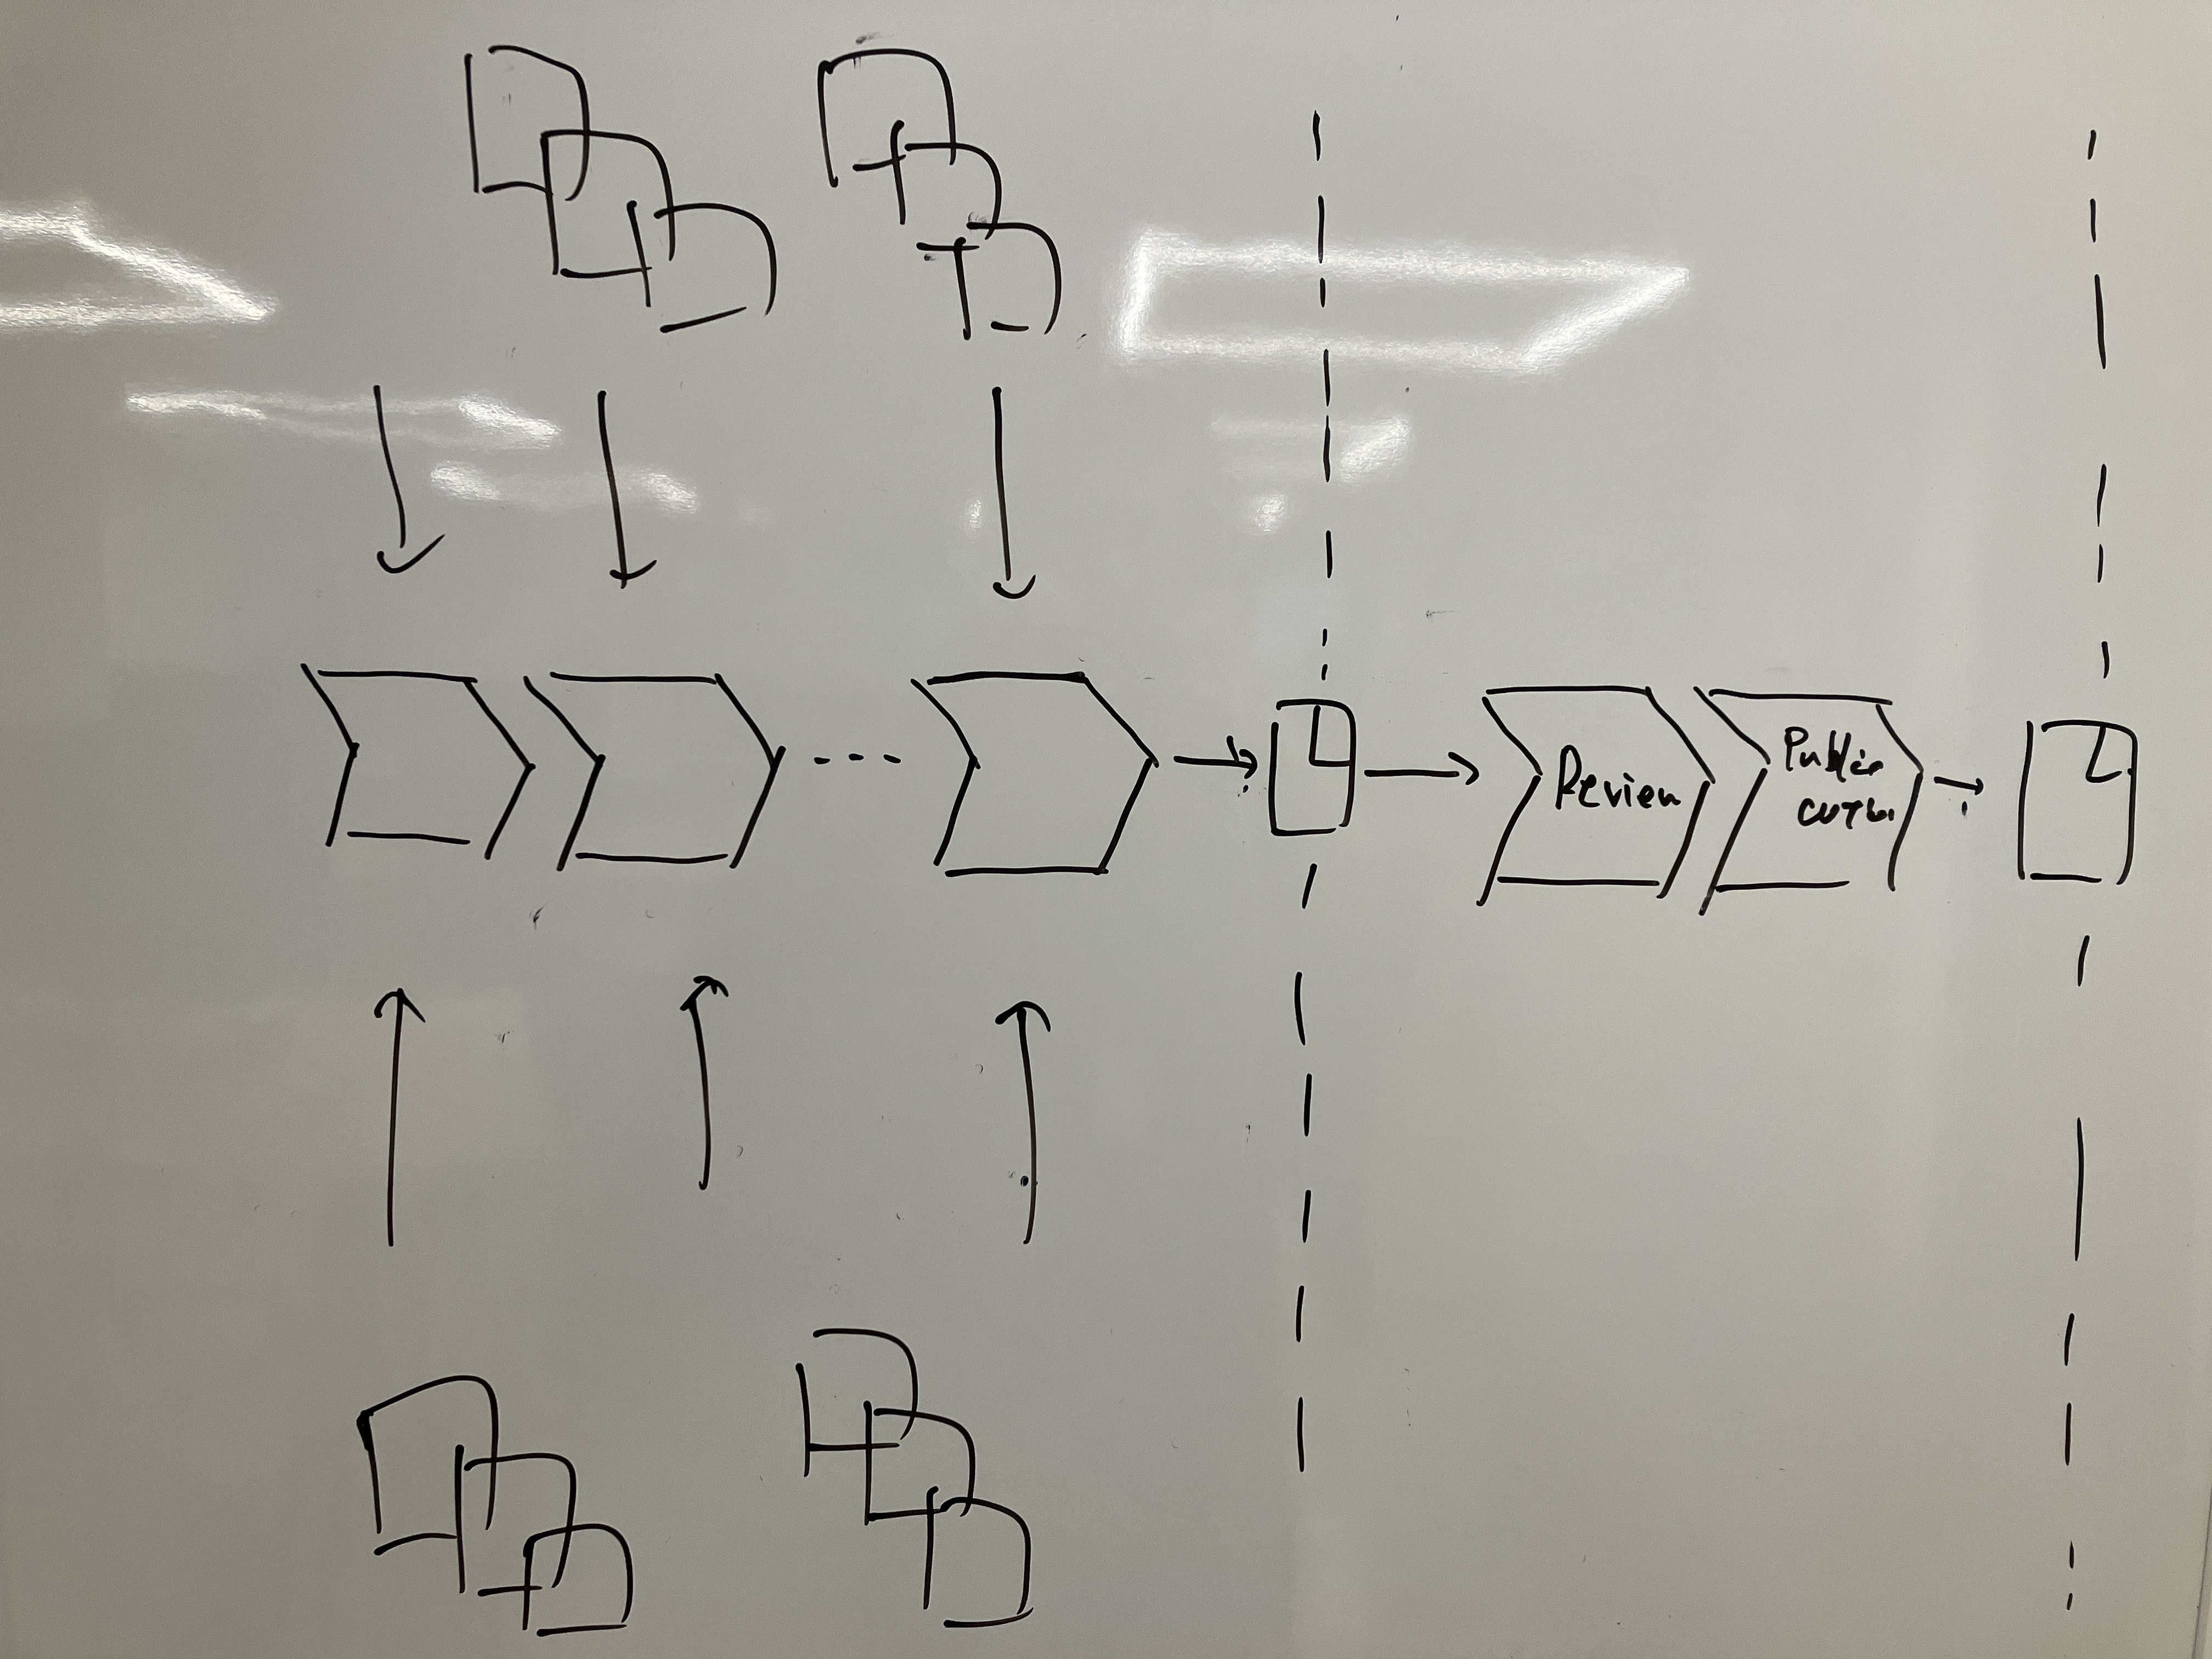
\includegraphics[width=\textwidth]{figs/researchprocess.jpg}
    \caption{Caption}
    \label{fig:research_process}
\end{figure}

This structuring is tentative and there may be a better way to structure the research process. However, I have created this structure for practical purposes in order to move the discussion forward. I will explain the reason for this division later. It is extremely important to consider research and, ultimately, the automation of research when thinking about better structuring. I hope the structure of this article be a starting point for conceiving a better structurization.

I will now proceed to a more detailed explanation of each step in the structured research process, followed by a separate discussion on reading and writing research papers.

\subsubsection{Topic Decision}
As mentioned earlier, research is an act of creating new knowledge. Usually, when people engage in research, they have a specific \textit{purpose} in mind before they decide what unknown they try to make known.

For example, let's say that someone proposes an algorithm that extends the reasoning capabilities of neural networks. This research may entails the thought process of ``I want to create artificial general intelligence, which requires reasoning capabilities, and for that we need to....'' In this case, the final purpose is to achieve ``artificial general intelligence'', and the research conducted as a result is ``proposing an algorithm that extends the reasoning capabilities of neural networks.'' Of course, this purpose may also be a means to achieve another purpose (such as intellectual curiosity), but since we cannot infinitely regress, we will assume that there is one purpose for one study.

In any case, there is gap between the purpose and the unknown we are trying to make known. We connect the sub-goals (, or sub-unknowns) by multi-step plausible inferences process.

\begin{figure}[htb]
    \centering
    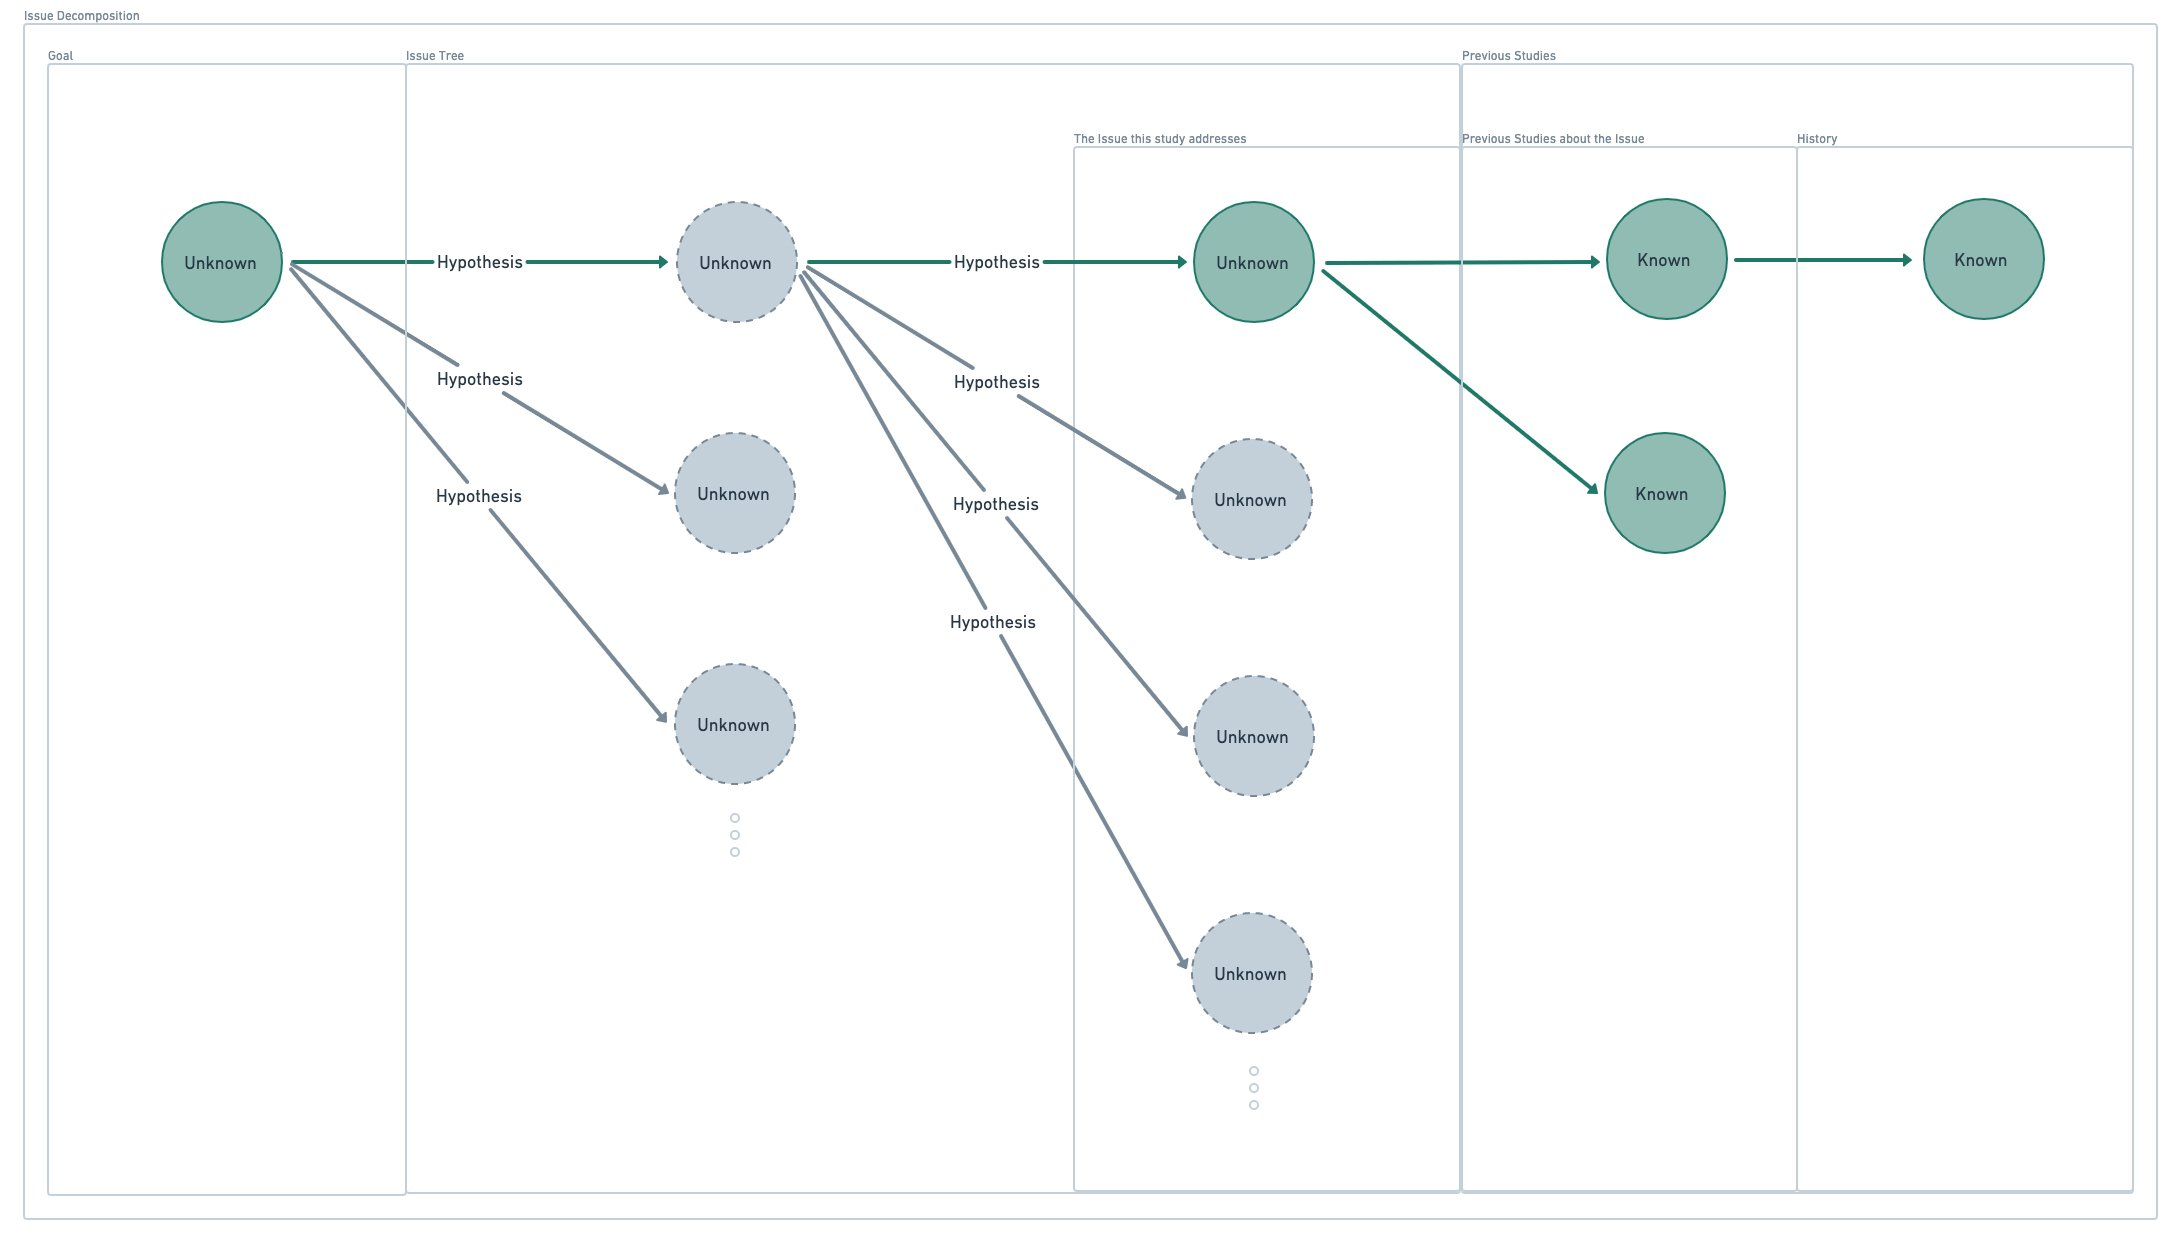
\includegraphics[width=\textwidth]{figs/unknown_tree.jpeg}
    \caption{Caption}
    \label{fig:unknown_tree}
\end{figure}


In other words, when humans engage in research, topic selection and issue identification are necessary.

\subsubsection{Hypothesis Generation}
Once the problem to be addressed has been identified, the next step is to generate a hypothesis. Research is an act of producing new knowledge, which can also be described as the act of converting the unknown to the known. Therefore, in research, inference about the unknown is inevitable. 

The scientific method, a methodology for knowledge production as previously mentioned, predominantly employs the hypothesis testing method. In this approach, a prediction about the unknown is explicitly stated as a hypothesis, and a procedure called verification is established to evaluate the validity of this hypothesis. Through this verification process, the evaluation of the hypothesis is conducted and the uncertainty towards the target unknown is reduced. This is the knowledge production based on the hypothesis testing method.

Hypotheses are often implicitly established even if they are not explicitly stated. Moreover, multiple hypotheses are often created in a study. For example, in mathematics, knowledge production is achieved through a deductive process called proof. However, when searching for lemmas to use in this process, we sometimes make predictions such as ``this lemma might be useful`` and examine it with specific examples. This may be considered as implicitly establishing a hypothesis and roughly verifying it. Therefore, even if the hypothesis testing method is not explicitly utilized, hypothesis generation is considered to be a very important part of research in nature.

In engineering research, as part of new knowledge, it is often required to propose actual design plans or algorithms. This can be considered as having a similar function to a hypothesis in the sense that it is a proposal for addressing a problem and is evaluated in some way.

In mathematical research, proving a theorem that was previously unknown is the production of knowledge. However, since mathematics is a deductive system, if the proof is correctly executed, it can be said to be ``correct'' in that sense. In other words, the proof itself is both the proposal and the verification. Therefore, mathematics is not a type of work that separates hypothesis and verification.

\subsubsection{Verification Design}
Once a hypothesis has been established, a verification plan is created to determine how to verify it. The specific method of verification depends on the subject being investigated, making this aspect of research difficult to structurize and automate in a unified way.

However, in many empirical sciences, the likelihood of a hypothesis is evaluated based on statistical significance. This is done by \textit{hypothesis testing} in practice. As this is a hypothesis test, it can only reject the null hypothesis, rather than directly determining the correctness of the hypothesis. Therefore, it can only be said that the hypothesis has survived for the time being. The belief that the surviving hypothesis is more likely to be valid is the basis for decision-making.

In any case, humans seem to use statistics or probability as the basis for assessing the validity of a hypothesis. In other words, we seem to concede to consider a hypothesis as plausible if something that cannot happen by chance, such as observing the same number repeatedly. This is based on the assumption of the ``principle of confirmation,`` which assumes that if the number of observations increases, it can be considered more reliable, and the ``principle of uniformity,`` which assumes that things will continue to proceed as they have been if the conditions remain the same. These beliefs ultimately serve as the basis for verification and scientific knowledge production. 

I will not delve into the validity of these beliefs here. What matters is that our research activity follow a practice that ``when a hypothesis is present, and a certain criterion and procedure are prepared, and the hypothesis is considered valid according to that procedure, we consider it valid.''

In theoretical research, sometimes there is no verification plan. Theory is a hypothesis, and its validity is determined separately through verification (not in the sense of whether it is mathematically valid, but for example whether it explains physical phenomena or not). However, in complex modern science, theorists propose a theory, and experimentalists verify it.

% Therefore, it is understood that in current research practice, shared knowledge in the form of papers may not necessarily provide a complete answer to a given question. This is similar to research on negative data. Negative data cannot solve the unknown initially declared, but it can reduce a certain degree of uncertainty towards it. This is because the validity of the presented hypothesis may have decreased somewhat. If this is the case, each research shared in the form of a paper may be more appropriate to describe as "reducing uncertainty towards the unknown," rather than "making the unknown known." This can become complicated when scrutinized strictly, so let's put this aside for now and continue to discuss how "producing new knowledge" is research.

In reality, conducting research is expected to be done with limited resources (time, funding, computing resources, people, etc.). Therefore, it is necessary to consider these resources when determining the verification approach. After a research design is determined at an abstract level, the feasibility of the research plan is roughly evaluated through a simple problem setting. This is known as a pilot study.
\subsubsection{Verification}

As mentioned earlier, in the case of empirical sciences, testing is often performed. Therefore, data is first generated, processed, and finally verified using the processed data. If we summarize the process of generating and processing raw data as data generation, this process can be broadly divided into data generation and judgment based on verification criteria. It may be rather said that the act of research itself is a process of repeatedly generating data and performing some kind of processing on it.

I separated the verification plan from the verification because I want to separate the description and execution of the process. The verification plan is analogous to coding, while the verification is more similar to executing the code.

The output of this process is usually wrtitten in the result section in the paper.

\subsubsection{Analysis}
At this stage, researchers interpret the results obtained from the verification. While the process leading up to the verification involved following a pre-determined procedure, researchers now consider implications that may relate to the unknown that they originally attempted to solve. For example, they contemplate whether the hypothesis has been rejected or the claim has been supported, and whether there are any other noteworthy points to consider. In papers, this stage is often described in discussion section.

\subsubsection{Paper Reading}
As previously mentioned, acquiring information from academic papers is a fundamental task necessary in all aspects of research.

In particular, there may be cases where one does not even know where to find the necessary knowledge. Therefore, in order to obtain the required information, it is necessary to first search for the academic papers themselves where the information is stored. 
Additionally, researchers sometimes have to compare multiple papers. Researchers need to demonstrate in the paper that the problem they are trying to solve is truly unknown, and that their proposal is truly novel.

A survey combines all of these tasks. In other words, it is the process of information retrieval and extraction from multiple academic papers followed by decision-making.
\subsubsection{Paper Writing}

Papers are assets, reports, and works.
``Importance'' is explained in a way that conveys information value to readers and makes them look attractive.

While academic papers are already structured into sections such as introduction, method, results, discussion, and conclusion, I believe that further sub-structuring of these sections could make it easier for readers to gather information. For example, the introduction section contains a broad range of elements, but breaking it down into more detailed subheadings could help readers more easily access the information they need.

There are various techniques for writing academic papers, but they are all designed with the assumption that humans will be reading the paper. Papers are considered to be ``reports'' and are expected to provide information to readers at a low cost. Additionally, papers are usually peer-reviewed and published in academic journals, so it is necessary to write attractive and engaging papers that will be accepted by the best journals. In this sense, papers are also ``works of art.'' However, I believe that the essential nature of papers lies in their role as the foundation of knowledge production, making papers an asset in terms of their ``knowledge'' aspect.

\subsubsection{Peer Review}
In current research, a small group of experts review papers and the results that pass through their review are publicly published. The review evaluates papers from multiple different perspectives. For example, at NeurIPS 2022, papers are evaluated based on the criterias of originality, quality, clarity, and significance.


\section{Research Automation}

Automation of abstract processes

Automation of individual concrete processes

\section{Proposal}

Proposal for the progress of automation of individual tasks

Automation of tasks and fundamentally autonomous (end-to-end) research

Proposal for the progress towards the realization of intelligence that can autonomously conduct research.

\section{Conclusion}

\end{document}